\documentclass{article}
\usepackage{fontspec,tikz,graphicx}
\setmainfont{Times New Roman}
\usepackage[a3paper,margin=1cm]{geometry}
\pagestyle{empty}
\begin{document}
\noindent\resizebox{\textwidth}{!}{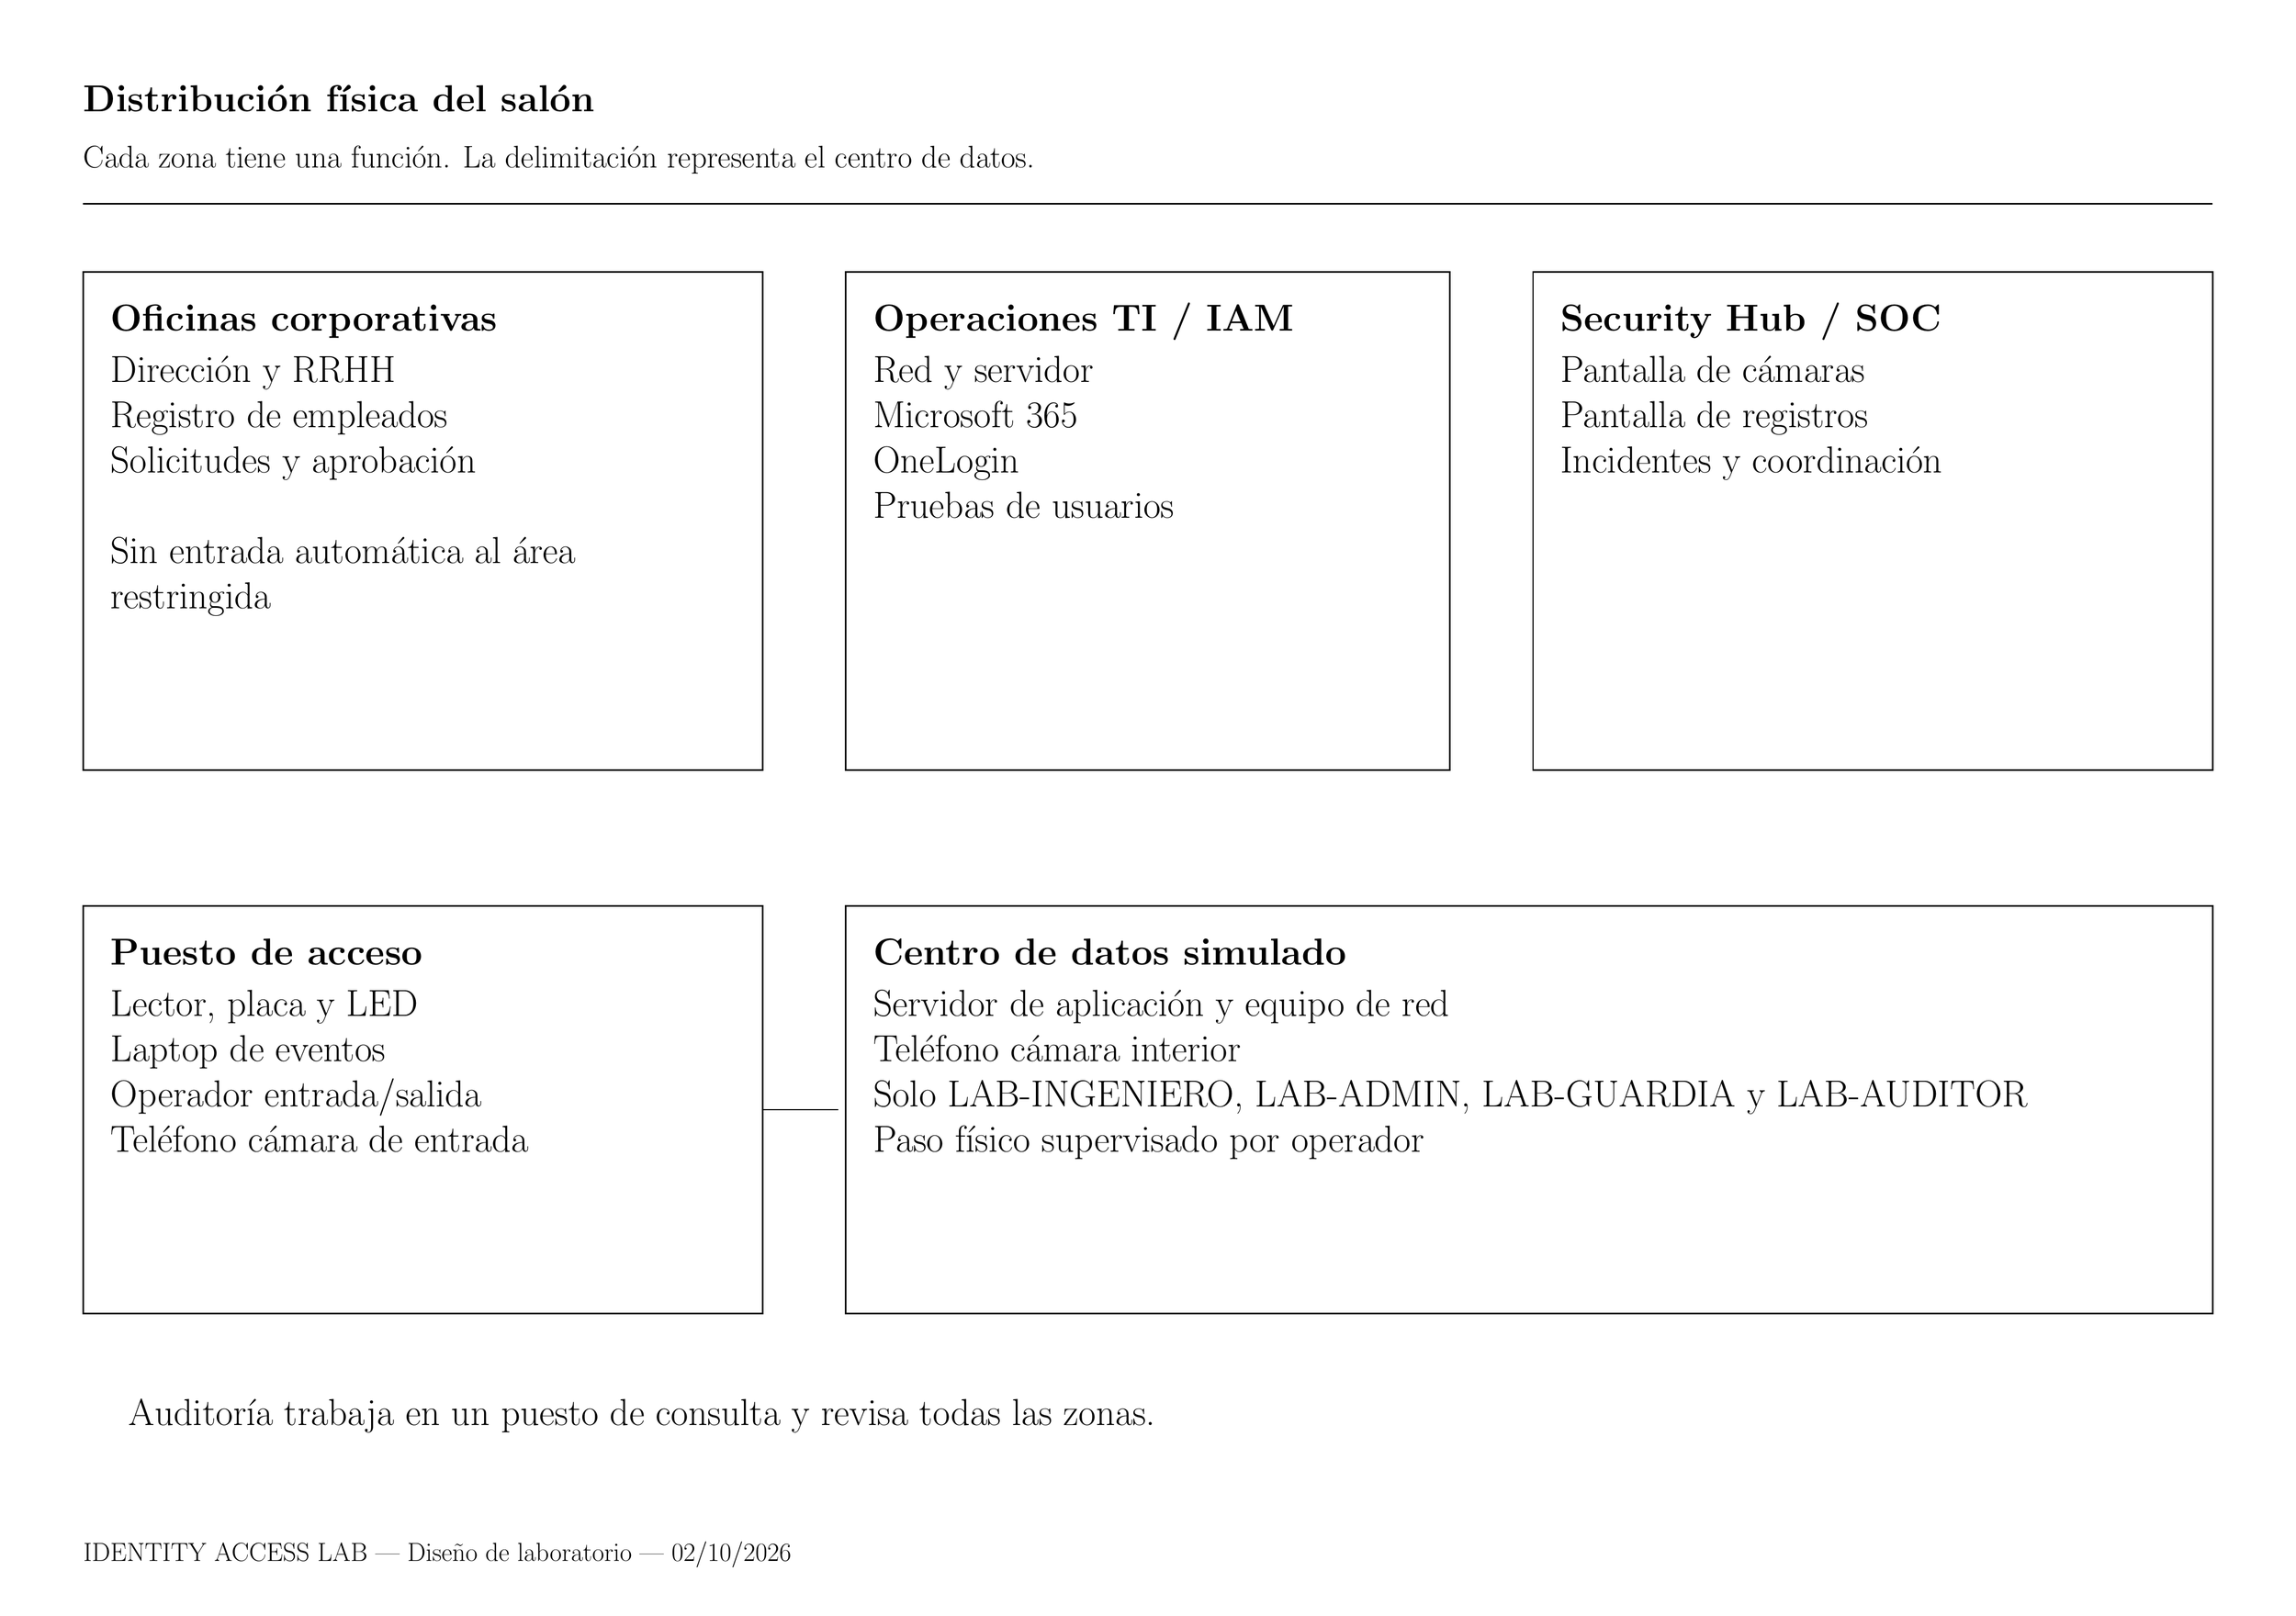
\begin{tikzpicture}[x=1pt,y=-1pt]
\path[use as bounding box] (0,0) rectangle (1500.0,1050.0);
\node[anchor=base west,inner sep=0pt,font=\fontsize{34.0}{40.8}\selectfont \bfseries ] at (45,64) {Distribución física del salón};
\node[anchor=base west,inner sep=0pt,font=\fontsize{21.0}{25.2}\selectfont ] at (45,101) {Cada zona tiene una función. La delimitación representa el centro de datos.};
\draw[line width=1pt] (45,125) -- (1455,125);
\draw[line width=1pt] (45.0,170.0) rectangle (495.0,500.0);
\node[anchor=base west,inner sep=0pt,font=\fontsize{25.0}{30.0}\selectfont \bfseries ] at (63,209) {Oficinas corporativas};
\node[anchor=base west,inner sep=0pt,font=\fontsize{23.0}{27.599999999999998}\selectfont ] at (63,243) {Dirección y RRHH};
\node[anchor=base west,inner sep=0pt,font=\fontsize{23.0}{27.599999999999998}\selectfont ] at (63,273) {Registro de empleados};
\node[anchor=base west,inner sep=0pt,font=\fontsize{23.0}{27.599999999999998}\selectfont ] at (63,303) {Solicitudes y aprobación};
\node[anchor=base west,inner sep=0pt,font=\fontsize{23.0}{27.599999999999998}\selectfont ] at (63,333) {};
\node[anchor=base west,inner sep=0pt,font=\fontsize{23.0}{27.599999999999998}\selectfont ] at (63,363) {Sin entrada automática al área};
\node[anchor=base west,inner sep=0pt,font=\fontsize{23.0}{27.599999999999998}\selectfont ] at (63,393) {restringida};
\draw[line width=1pt] (550.0,170.0) rectangle (950.0,500.0);
\node[anchor=base west,inner sep=0pt,font=\fontsize{25.0}{30.0}\selectfont \bfseries ] at (568,209) {Operaciones TI / IAM};
\node[anchor=base west,inner sep=0pt,font=\fontsize{23.0}{27.599999999999998}\selectfont ] at (568,243) {Red y servidor};
\node[anchor=base west,inner sep=0pt,font=\fontsize{23.0}{27.599999999999998}\selectfont ] at (568,273) {Microsoft 365};
\node[anchor=base west,inner sep=0pt,font=\fontsize{23.0}{27.599999999999998}\selectfont ] at (568,303) {OneLogin};
\node[anchor=base west,inner sep=0pt,font=\fontsize{23.0}{27.599999999999998}\selectfont ] at (568,333) {Pruebas de usuarios};
\draw[line width=1pt] (1005.0,170.0) rectangle (1455.0,500.0);
\node[anchor=base west,inner sep=0pt,font=\fontsize{25.0}{30.0}\selectfont \bfseries ] at (1023,209) {Security Hub / SOC};
\node[anchor=base west,inner sep=0pt,font=\fontsize{23.0}{27.599999999999998}\selectfont ] at (1023,243) {Pantalla de cámaras};
\node[anchor=base west,inner sep=0pt,font=\fontsize{23.0}{27.599999999999998}\selectfont ] at (1023,273) {Pantalla de registros};
\node[anchor=base west,inner sep=0pt,font=\fontsize{23.0}{27.599999999999998}\selectfont ] at (1023,303) {Incidentes y coordinación};
\draw[line width=1pt] (45.0,590.0) rectangle (495.0,860.0);
\node[anchor=base west,inner sep=0pt,font=\fontsize{25.0}{30.0}\selectfont \bfseries ] at (63,629) {Puesto de acceso};
\node[anchor=base west,inner sep=0pt,font=\fontsize{23.0}{27.599999999999998}\selectfont ] at (63,663) {Lector, placa y LED};
\node[anchor=base west,inner sep=0pt,font=\fontsize{23.0}{27.599999999999998}\selectfont ] at (63,693) {Laptop de eventos};
\node[anchor=base west,inner sep=0pt,font=\fontsize{23.0}{27.599999999999998}\selectfont ] at (63,723) {Operador entrada/salida};
\node[anchor=base west,inner sep=0pt,font=\fontsize{23.0}{27.599999999999998}\selectfont ] at (63,753) {Teléfono cámara de entrada};
\draw[line width=1pt] (550.0,590.0) rectangle (1455.0,860.0);
\node[anchor=base west,inner sep=0pt,font=\fontsize{25.0}{30.0}\selectfont \bfseries ] at (568,629) {Centro de datos simulado};
\node[anchor=base west,inner sep=0pt,font=\fontsize{23.0}{27.599999999999998}\selectfont ] at (568,663) {Servidor de aplicación y equipo de red};
\node[anchor=base west,inner sep=0pt,font=\fontsize{23.0}{27.599999999999998}\selectfont ] at (568,693) {Teléfono cámara interior};
\node[anchor=base west,inner sep=0pt,font=\fontsize{23.0}{27.599999999999998}\selectfont ] at (568,723) {Solo LAB-INGENIERO, LAB-ADMIN, LAB-GUARDIA y LAB-AUDITOR};
\node[anchor=base west,inner sep=0pt,font=\fontsize{23.0}{27.599999999999998}\selectfont ] at (568,753) {Paso físico supervisado por operador};
\draw[line width=1pt] (495,725) -- (545,725);
\node[anchor=base west,inner sep=0pt,font=\fontsize{24.0}{28.799999999999997}\selectfont ] at (75,934) {Auditoría trabaja en un puesto de consulta y revisa todas las zonas.};
\node[anchor=base west,inner sep=0pt,font=\fontsize{18.0}{21.599999999999998}\selectfont ] at (45,1024) {IDENTITY ACCESS LAB | Diseño de laboratorio | 02/10/2026};
\end{tikzpicture}}
\end{document}
